\section{Introduzione}\label{intro}

Gli articoli scientifici sono materiale continuamente letto, richiesto e aggiornato in ambito universitario. Per questo motivo risulta interessante lo studio di funzionalità per estrarre i metadati da essi. Per metadati si intende l'insieme di descrittori del pdf quali: titolo, autore, tematica, parole chiavi.\\ In PDF supporterebbe uno standard predefinito per la descrizione di metadati, come mostrato in Figura \ref{fig:standard}, purtroppo l'eterogeneità dei tool di generazione PDF fa sì che non venga rispettato, lasciando vana la speranza di reperire le informazioni attraverso essi. Inoltre ci sono metadati come la bibliografia che non sono contemplati dallo standard. Per questi motivi si è reso necessario realizzare metodi che analizzassero il PDF a livello testuale per estrarli.\\

\begin{figure}[htb]
\begin{center}
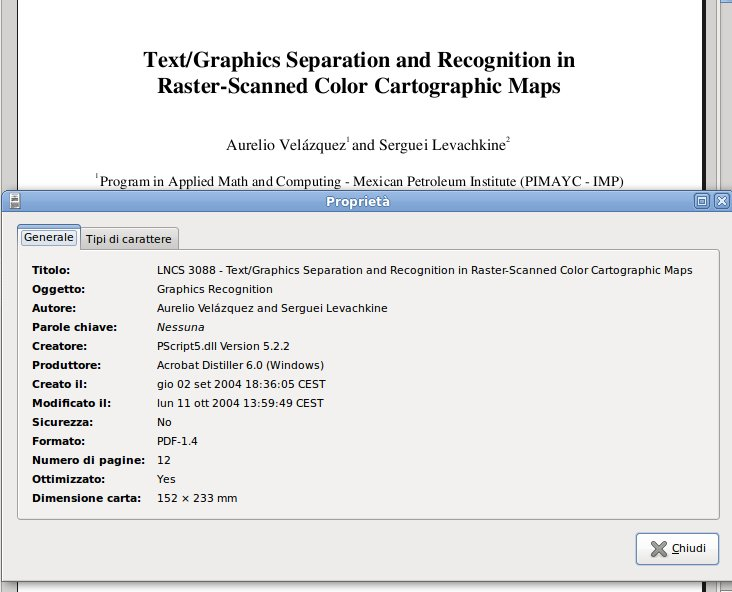
\includegraphics[scale=0.45]{pdf-standard.jpg}
\end{center}
\caption[Un esempio PDF che supporta alcuni metadati]{Un esempio PDF che supporta alcuni metadati mostrati nel lettore Evince della suite GNOME su GNU/Linux. Questi valori possono essere letti facilmente tramite qualsiasi libreria che gestisca il formato PDF, il problema sta nel fatto che non tutti i pdf sono benformati.}
\label{fig:standard}
\end{figure}


Durante l'esame del corso di \textit{Data Base II} è stato studiato il processo di Information Retrieval al fine di estrarre metadati, correlandoli con i rispettivi documenti in una biblioteca digitale come ad esempio Greenstone. Purtroppo come detto precentemente, l'estrazione dei metadati non è un processo standardizzato, è stato perciò necessario elaborare un processo di analisi del testo del documento PDF, sfruttando le nozioni del corso. In questo senso l'elaborato si colloca come un approfondimento al corso utile a sviluppare un certo senso critico riguardo l' Information Retrieval.\\
L'attenzione si è focalizza sulla bibliografia, ispirandosi ad alcuni elaborati che erano già stati effettuati su estrazione di titolo e autore da articoli scientifici \cite{Tarocchi}. La bibliografia, \textit{references} in  termini anglosassoni, è definita dai riferimenti bibliografici come l'insieme dei documenti consultati e usati dall'autore per scrivere il suo articolo originale. In ogni articolo alla fine si trova la lista dei riferimenti spesso accompagnata da una numerazione che abbina l'articolo alla parte citata nel testo.
\\ 
Un caso d'uso possibile potrebbe essere quello in cui un ricercatore vorrebbe ottenere immediatamente dei riferimenti online relativi ad una risorsa citata in un articolo che sta leggendo, per approfondire una certa tematica. A partire da questa idea si è pensato ad un modo per estrarre la bibliografia dall' articolo, ottenere le risorse Web collegate a ciascuna voce, riportare dove presente il codice BibTex associato e se possibile scaricare in locale l'articolo citato in formato PDF, per la consultazione \textit{offline}.

\'E facile capire come da un singolo articolo si crei una fitta rete di collegamenti ad altri articoli che a loro volta contengono altre citazioni. Risulta perciò interessante percorrere ricorsivamente l'intero grafo che collega l'un con l'altro i vari articoli. In ultima analisi la bibliografia è un oggetto particolare che rappresenta il collante tra articoli che con molta probabilità condividono il medesimo tema di fondo; un esempio di bibliografia può essere quello riportato in Figura \ref{fig:ref-examples}, che presenta una precisa numerazione.
\\
In questo senso sarebbe interessante provare a sviluppare un \textit{crawler} che dati in input una serie di articoli cerchi di indicizzare quelli che trova per collegamento, impostando eventualmente una certa profondità di ricerca, in maniera da costruirsi anche visivamente il grafo dei collegamenti tra gli articoli. Questa parte non è trattata nel nostro elaborato e sarà approfondita nella sezione degli sviluppi futuri. L'applicazione ottenuta con questo elaborato potrebbe essere usata sia come applicazione \textit{standalone} che integrata come ``motore'' di un crawler. Essa analizza un insieme di file pdf in input, cerca di estrarre la bibliografia evidenziandone i titoli e genera un file html con i metadati estratti per ogni documento di partenza. 


Nel seguito saranno spiegate nella sezione \ref{obiettivi} l'obiettivo dell'elaborato insieme ai problemi risolti, già citati nell'introduzione. L'elaborato ha dato alla luce un programma chiamato \textit{\htmladdnormallink{pdftoref}{http://code.google.com/p/pdftoref}} che si occupa dell'estrazione automatizzata dellla bibliografia. Nelle sezioni seguenti sarà spiegato come si è affronata l'analisi del problema, lo sviluppo dell'applicativo (sezione \ref{software} ) e infine i risultati ottenuti (sezione \ref{esperimenti} ) insieme alle conclusioni che ci hanno permesso di trarre (sezione \ref{conclusioni} ).


\begin{figure}[htb]
\begin{center}
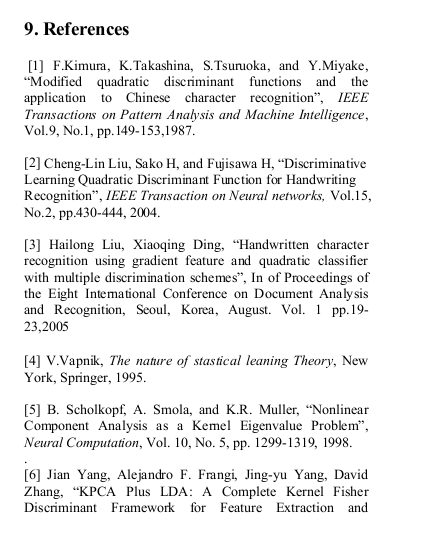
\includegraphics[scale=0.45]{ref.png}
\end{center}
\caption[Un esempio di bibliografia]{Un esempio di bibliografia estratte dall'articolo di una conferenza di ICDAR. E'subito intuitivo notare che la numerazione con parentesi quadre può costituire un ottimo punto di partenza per riuscire a capire quando inizia una nuova voce della bibliografia rispetto ad un'altra.}
\label{fig:ref-examples}
\end{figure}



